% !TEX root = ../../Main.tex
\section{Alpha and Beta Decomposition}
\label{Section:AlphaBeta}

A currency pair moves on its own. An agent that is long a pair that happens to rise will show a profit that has nothing to do with the policy it learned. The same is true for an agent that is short a pair that happens to fall. Total return cannot separate this profit from the profit of the policy. The results are therefore decomposed into the part explained by the market and the part that is not.

For each pair, the yearly return of the model is regressed on the yearly move of the pair itself, over the eleven years from 2015 to 2025. With $r_i$ the model return in year $i$ and $m_i$ the market move in the same year, ordinary least squares gives

\begin{equation}
\beta = \frac{\sum_i (m_i - \bar{m})(r_i - \bar{r})}{\sum_i (m_i - \bar{m})^2}, \qquad \alpha = \bar{r} - \beta \bar{m}
\label{Equation:AlphaBeta}
\end{equation}

$\beta$ measures the model's exposure to the market's movement. $\alpha$ is the average yearly return that is left once that exposure is removed. The mean return then splits into an active part and a passive part:

\begin{equation}
\bar{r} = \underbrace{\alpha}_{\text{policy}} + \underbrace{\beta \bar{m}}_{\text{market exposure}}
\label{Equation:AlphaDecomposition}
\end{equation}

Yearly returns are used instead of daily returns for a specific reason. The agents hold positions for days to weeks and act once a day. A daily regression would therefore measure how the model tracks the market within a holding period. It would not measure whether the model chose the right direction over the horizon it trades. Eleven yearly observations are a small sample, and each regression coefficient has a large uncertainty. The decomposition is good enough to sort the pairs into groups, but it does not give a precise value for any one of them.

\Cref{Tables:AlphaBeta} gives both terms. Six of the seven pairs have positive alpha, and the seven fall into three clear groups.

% !TEX root = ../Main.tex
\begin{table}[htb!]
\centering
\footnotesize
\caption{Decomposition of \Cref{Equation:AlphaDecomposition}, from the yearly regression of \Cref{Equation:AlphaBeta} over 2015 to 2025. Alpha is the return attributable to the policy, and the beta return is the part explained by the pair's own movement. The two add up to the mean yearly return.}
\label{Tables:AlphaBeta}
\begin{tabular}{@{}lrrrrl@{}}
\toprule
\textbf{Pair} & \textbf{Beta} & \textbf{Alpha (\%/yr)} & \textbf{Beta Return (\%/yr)} & \textbf{Mean (\%/yr)} & \textbf{Reading} \\
\midrule
AUD/USD & $-2.013$ & $+4.96$ & $+3.22$ & $+8.18$ & Policy plus leveraged trend \\
EUR/USD & $+0.266$ & $+6.62$ & $+0.01$ & $+6.63$ & Policy, no market exposure \\
GBP/USD & $-0.054$ & $+11.64$ & $+0.06$ & $+11.70$ & Policy, no market exposure \\
NZD/USD & $-0.708$ & $+2.79$ & $+1.83$ & $+4.62$ & Policy plus leveraged trend \\
USD/CAD & $+2.393$ & $+10.02$ & $+4.21$ & $+14.23$ & Policy plus leveraged trend \\
USD/CHF & $-0.082$ & $+3.91$ & $+0.16$ & $+4.07$ & Policy, no market exposure \\
USD/JPY & $+1.012$ & $-1.08$ & $+2.64$ & $+1.57$ & No policy; the model follows the market \\
\bottomrule
\end{tabular}
\end{table}

\textbf{Three pairs have almost no market exposure.} GBP/USD, EUR/USD and USD/CHF have betas of $-0.054$, $+0.266$ and $-0.082$. Their market exposure adds $0.06$, $0.01$ and $0.16$ percentage points per year to their returns. For GBP/USD, $11.64$ of its $11.70$ points per year come from the policy. These results would hold up if the market changed direction, because they hardly depend on the direction of the market.

\textbf{Three pairs combine policy with leveraged exposure.} USD/CAD at $+2.393$, AUD/USD at $-2.013$ and NZD/USD at $-0.708$ all have a large exposure to their market, and two of them are leveraged more than two to one. Their alpha is positive in every case, so the policy adds skill on top. But between a fifth and two fifths of what they earned came from the market moving in the direction of their exposure. USD/CAD is the clearest example: $4.21$ of its $14.23$ points per year came from the pair rising while the agent was net long. If the Canadian Dollar had become stronger over the decade instead, that component would have been a loss of similar size, and the reported $+226.6\%$ would look very different.

\Cref{Figure:AlphaBeta} plots the seven together, and the three groups are clearly separate.

\textbf{One pair has no policy at all.} USD/JPY has a beta of $+1.012$ and a correlation of $+0.946$ with its own market, and its alpha is $-1.08\%$ per year, the only negative figure in the table. It is examined in \Cref{Section:NegativeResult}.

\begin{figure}[htb!]
\centering
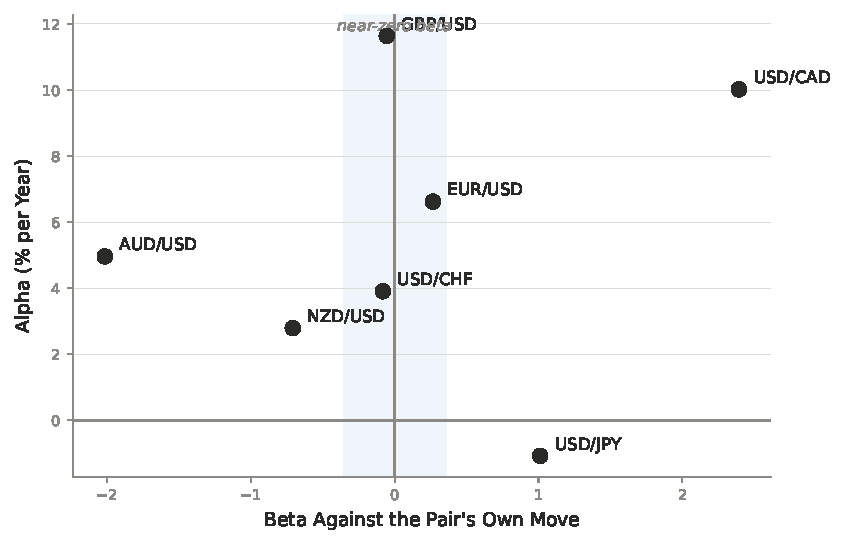
\includegraphics[width=0.82\textwidth]{Images/AlphaBeta.pdf}
\caption{Alpha against beta for the seven agents. Points inside the shaded band have almost no market exposure, so their return is attributable to the policy. USD/JPY sits at a beta of one with negative alpha. This is the pattern of a model that has copied its own market.}
\label{Figure:AlphaBeta}
\end{figure}

The method was checked before it was used. The same regression, run on the model of the previous campaign, reproduces its recorded figures exactly: a correlation of $+0.115$, a beta of $+0.130$ and an alpha of $+3.11\%$ per year. This confirms that the decomposition here is computed in the same way as the one it is compared with.

This decomposition is given priority over total return, for a reason that affects how the whole chapter should be read. The model to publish was chosen from a pool of candidates, and any measure used to make that choice is inflated by it. Return is such a measure. Beta is not. Beta describes how a policy behaves against its market. Selection can give a model a high return by luck, but it cannot give it a low beta in the same way. A large alpha with a beta near zero is therefore a stronger claim than a large return, and it is the claim this work puts first.